%% Author_tex.tex
%% V1.0
%% 2012/13/12
%% developed by Techset
%%
%% This file describes the coding for modeloUFCG.cls

\documentclass[a4paper]{modeloUFCG} %%%% where modeloUFCG is the template name

\usepackage[portuguese]{babel}
\usepackage[T1]{fontenc}
\usepackage[utf8]{inputenc}
\usepackage{fancyhdr}
\usepackage{booktabs}
\usepackage{longtable}
\usepackage{array}
\usepackage{calc}
%% Fixa cada figura exatamente onde e gerada ([H]). Sem isso, floats podem
%% "flutuar" livremente e, neste documento (muitas figuras grandes em
%% sequencia), acabam se deslocando para muito longe do texto que os
%% referencia -- inclusive interferindo na quebra de pagina de tabelas
%% longtable vizinhas.
\usepackage{float}

%% A classe modeloUFCG.cls calcula largura/altura de texto e margens
%% assumindo o formato de trim de um periodico (174mm x 247mm), mas o PDF
%% final e produzido em A4 (210mm x 297mm). Isso deixa sobras enormes nas
%% margens. O pacote geometry forca margens A4 corretas, sobrepondo o
%% calculo original da classe.
\usepackage[a4paper, margin=2.5cm]{geometry}

\pagestyle{fancy}
\renewcommand{\headrulewidth}{0pt}
\fancyhead[L]{}
\fancyhead[C]{}
\fancyhead[R]{}

%% A classe usa \flushbottom, que estica os espacos em branco de cada pagina
%% para preenche-la ate o final. Combinado com figuras fixas ([H]), isso cria
%% buracos enormes entre uma figura/tabela e o texto seguinte. \raggedbottom
%% deixa o espaco sobrando apenas no rodape da pagina, sem esticar o meio.
\raggedbottom

%% Espacamento mais enxuto ao redor de figuras e tabelas.
\setlength{\floatsep}{8pt plus 2pt minus 2pt}
\setlength{\textfloatsep}{10pt plus 2pt minus 2pt}
\setlength{\intextsep}{8pt plus 2pt minus 2pt}


%%%% *** Do not adjust lengths that control margins, column widths, etc. ***

%%%%%%%%%%% Defining Enunciations  %%%%%%%%%%%
\newtheorem{theorem}{\bf Teorema}[section]
\newtheorem{condition}{\bf Condição}[section]
\newtheorem{corollary}{\bf Corolário}[section]
%%%%%%%%%%%%%%%%%%%%%%%%%%%%%%%%%%%%%%%%%%%%%%%

\usepackage{titlesec}
\renewcommand{\thesection}{\arabic{section}}
\renewcommand{\thesubsection}{\thesection.\arabic{subsection}}
\renewcommand{\thesubsubsection}{\thesubsection.\arabic{subsubsection}}

%%%% Cabecalho no estilo de artigo academico, substituindo a capa           %%%%
%%%% original (logo + caixa de titulo) do template Royal Society.          %%%%
%%%% A caixa de resumo estreita e trocada por um resumo de largura total,  %%%%
%%%% exibido logo apos o titulo/autores, como em um artigo convencional.   %%%%
%% Apos o \documentclass terminar de carregar, o LaTeX restaura o catcode de
%% @ para "outro", entao qualquer referencia a comandos internos da classe
%% (\@title, \@author, \if@subject@provided etc.) precisa ficar dentro de
%% \makeatletter ... \makeatother para ser reconhecida corretamente.
\makeatletter

%% Centraliza as legendas de figuras e tabelas (a classe original as deixa
%% alinhadas a esquerda).
\long\def\@makecaption#1#2{%
  \vskip\abovecaptionskip
  \centering{\captionheadfont #1.}\hskip2.5pt{\captionfont #2}\par
  \vskip\belowcaptionskip}

\renewenvironment{abstract}{%
  \global\setbox\absbox\vbox\bgroup\par\abstractfont
  \leftskip0pc\rightskip0pc\noindent\ignorespaces
}{\par\egroup}

%% A classe modeloUFCG.cls define \@maketitle atraves de mecanismos internos
%% (fila de duas colunas / bloco de revisao editorial) que absorvem qualquer
%% redefinicao de \@maketitle sem executa-la. Para evitar essa maquinaria,
%% \maketitle e redefinido diretamente aqui.
\renewcommand\maketitle{%
  \vspace*{-2.2cm}
  \noindent\begin{minipage}[c]{2.2cm}
    
\includegraphics[width=2cm]{lea_logo_bw}
  \end{minipage}%
  \begin{minipage}[c]{\textwidth-2.2cm}
    {\fontfamily{\sfdefault}\fontseries{b}\fontshape{n}\fontsize{12}{14}\selectfont
      UNIVERSIDADE FEDERAL DE CAMPINA GRANDE\par}
          {\fontfamily{\sfdefault}\fontseries{m}\fontshape{n}\fontsize{11}{13}\selectfont
       Disciplina: Estatística Aplicada%
        \quad---\quad Período: 2026.1\par}
              {\fontfamily{\sfdefault}\fontseries{m}\fontshape{n}\fontsize{11}{13}\selectfont
       Professores: Profa. Dra. Amanda Gomes; Prof.~Dr.~Jerfson Bruno; Prof.~Dr.~Gilberto Matos\par}
      \end{minipage}
  \vskip4pt
  \rule{\textwidth}{.5pt}
  \vskip8pt
  \begin{center}
    {\fontfamily{\sfdefault}\fontseries{m}\fontshape{n}\fontsize{16}{18}\selectfont\mathversion{bold}\@title\par}
    \vskip6pt
    {\authorfont\@author\par}
    \vskip3pt
    \ifx\@address\empty\else
      {\addressfont\@address\par}
    \fi
    \vskip6pt
    \rule{\textwidth}{.5pt}
  \end{center}
  \vskip8pt
  \ifvoid\absbox\else
    {\fontfamily{\sfdefault}\fontseries{b}\fontshape{n}\fontsize{11}{13}\selectfont Resumo}\par
    \vskip4pt
    \noindent\usebox\absbox\par
    \vskip6pt
  \fi
  \if@subject@provided
    {\subjectfont\@subject\par}
    \vskip4pt
  \fi
  \if@keywords@provided
    {\keywordfont\@keywords\par}
  \fi
  \vskip10pt
}

\makeatother

\begin{document}

%%%% Article title to be placed here
\title{Modelagem da Relação de Vendas de Cadeirinhas Infantis}

\author{
Kayo$^{Salvino}$,
José Ryan Santos de Melo$^{}$,
Hugo$^{Silva}$}

\address{
  $^{}$Departamento de Ciência da Computação - UFCG}
%%%% Subject entries to be placed here %%%%
\subject{
estatistica aplicada,
modelagem preditiva,
inferencia estatistica}

%%%% Keyword entries to be placed here %%%%
\keywords{
regressao linear multipla,
testes de hipotese,
intervalos de confianca,
selecao de modelos,
analise de vendas}

%%%% Abstract text to be placed here %%%%%%%%%%%%
\begin{abstract}
Este trabalho aplica a Regressão Linear Múltipla (RLM) para modelar o volume de vendas de cadeirinhas infantis (Sales) a partir da base de dados Carseats. O objetivo principal é quantificar o impacto de fatores como precificação, investimento em publicidade, perfil demográfico e exposição do produto no desempenho de vendas em 400 lojas, com foco na inferência estatística. A metodologia abrange uma análise exploratória preliminar, seguida pelo ajuste do modelo e pela avaliação da significância das variáveis explicativas por meio de testes de hipótese individuais e em conjunto . Além disso, o estudo constrói intervalos de confiança para os coeficientes, seleciona um modelo final ajustado e calcula intervalos de confiança e de predição para cenários hipotéticos. Dessa forma, o relatório vai além da predição, oferecendo uma interpretação prática e fundamentada das dinâmicas comerciais no varejo.
\end{abstract}
%%%%%%%%%%%%%%%%%%%%%%%%%%%

%% Some pieces required from the pandoc template
\providecommand{\tightlist}{%
  \setlength{\itemsep}{0pt}\setlength{\parskip}{0pt}}
\providecommand{\EndFirstPage}{%
}

\maketitle

\section{Introdução}\label{introduuxe7uxe3o}

A previsão do volume de vendas de um produto a partir de fatores como preço, concorrência, publicidade e características demográficas da região de venda constitui um problema recorrente em análises de varejo. A base Carseats, com dados simulados de vendas de cadeirinhas infantis em 400 lojas, permite ilustrar como esses fatores --- precificação própria e da concorrência, investimento em publicidade, perfil socioeconômico da região (renda, população, idade, escolaridade) e a qualidade da exposição do produto na prateleira --- se relacionam com o desempenho de vendas, e como essa relação pode ser quantificada e testada estatisticamente.

Neste trabalho, o objetivo é modelar as vendas (Sales, em milhares de unidades) a partir das demais variáveis disponíveis na base, utilizando regressão linear múltipla (RLM) como ferramenta central de análise. Mais do que ajustar um modelo preditivo, o interesse do trabalho está em aplicar, sobre os coeficientes estimados, os instrumentos de inferência estatística estudados na disciplina: testes de hipótese sobre a significância de cada variável explicativa e intervalos de confiança para os parâmetros do modelo e para o valor médio esperado da resposta.

Especificamente, buscamos: (i) descrever a base de dados e realizar uma análise exploratória uni e bivariada; (ii) ajustar um modelo de regressão linear múltipla com as variáveis explicativas disponíveis; (iii) testar formalmente a significância de cada coeficiente por meio de testes de hipótese individuais (teste \(t\)) e da significância conjunta do modelo (teste \(F\)); (iv) construir intervalos de confiança para os coeficientes estimados, interpretando seu significado prático; (v) selecionar um modelo final com base nesses resultados; e (vi) apresentar, para valores hipotéticos das variáveis explicativas, os intervalos de confiança para o valor médio esperado das vendas e os intervalos de predição para uma nova observação, discutindo a diferença entre ambos.

\subsection{Modelo de regressão linear múltipla}\label{modelo-de-regressuxe3o-linear-muxfaltipla}

A ideia da regressão linear múltipla é explicar uma variável resposta \(Y\) (no nosso caso, Sales, o volume de vendas em milhares de unidades) a partir de várias variáveis explicativas ao mesmo tempo, supondo que a relação entre elas é (aproximadamente) uma soma ponderada:

\[
Y_i = \beta_0 + \beta_1 X_{i1} + \beta_2 X_{i2} + \cdots + \beta_{p-1} X_{i,p-1} + \varepsilon_i
\]

em que \(\beta_0\) é o intercepto, cada \(\beta_j\) mede o efeito da variável \(X_j\) sobre as vendas (mantendo as outras variáveis fixas) e \(\varepsilon_i\) é o erro, ou seja, a parte das vendas que o modelo não consegue explicar. Usando todas as variáveis da base Carseats, o modelo fica:

\[
\begin{aligned}
\text{Sales}_i = \ \beta_0 &+ \beta_1\, \text{CompPrice}_i + \beta_2\, \text{Income}_i + \beta_3\, \text{Advertising}_i + \beta_4\, \text{Population}_i \\
&+ \beta_5\, \text{Price}_i + \beta_6\, \text{ShelveLocGood}_i + \beta_7\, \text{ShelveLocMedium}_i + \beta_8\, \text{Age}_i \\
&+ \beta_9\, \text{Education}_i + \beta_{10}\, \text{UrbanYes}_i + \beta_{11}\, \text{USYes}_i + \varepsilon_i
\end{aligned}
\]

ShelveLocGood e ShelveLocMedium indicam se a exposição do produto é boa ou média (a categoria ``Bad'' fica implícita no intercepto), e UrbanYes/USYes indicam se a loja é urbana e se é dos EUA (a categoria ``Não'' fica implícita).

Os \(\beta_j\) são estimados pelo método dos mínimos quadrados, que escolhe a reta (ou ``plano'') que minimiza a soma dos quadrados dos erros de previsão. Para que os testes de hipótese e os intervalos de confiança que vamos usar façam sentido, o modelo assume que:

\begin{itemize}
\tightlist
\item
  a relação entre as variáveis e as vendas é de fato aproximadamente linear;
\item
  os erros, em média, valem zero (o modelo não erra sistematicamente para cima ou para baixo);
\item
  os erros têm variância parecida em toda a faixa de valores (não erra muito mais para lojas grandes do que para pequenas, por exemplo);
\item
  os erros de uma loja não influenciam o erro de outra;
\item
  os erros seguem aproximadamente uma distribuição normal;
\item
  as variáveis explicativas não são muito redundantes entre si (isto será checado mais à frente com o VIF).
\end{itemize}

\subsection{Testes de hipótese e intervalos de confiança}\label{testes-de-hipuxf3tese-e-intervalos-de-confianuxe7a}

Depois de ajustar o modelo, queremos saber quais variáveis realmente importam para explicar as vendas. Para cada coeficiente \(\beta_j\), fazemos um teste de hipótese:

\[
H_0: \beta_j = 0 \quad \text{vs} \quad H_1: \beta_j \neq 0
\]

Ou seja, \(H_0\) diz que a variável não tem efeito nenhum sobre as vendas. A estatística de teste é

\[
t_j = \frac{\hat{\beta}_j}{\text{ep}(\hat{\beta}_j)}
\]

que compara o tamanho do coeficiente estimado com o seu erro padrão. Quanto maior (em módulo) esse \(t_j\), mais evidência temos de que a variável realmente tem efeito. Na prática, olhamos o p-valor: se for menor que 0,05, rejeitamos \(H_0\) e dizemos que a variável é estatisticamente significante.

Além de testar cada variável separadamente, existe um teste para saber se o modelo como um todo é útil --- o teste \(F\):

\[
H_0: \beta_1 = \beta_2 = \cdots = \beta_{p-1} = 0
\]

isto é, nenhuma das variáveis explica as vendas. Se o p-valor do teste \(F\) for pequeno, rejeitamos essa hipótese e concluímos que pelo menos uma variável do modelo ajuda a explicar as vendas.

Também calculamos intervalos de confiança para cada \(\beta_j\), que dão uma faixa de valores plausíveis para o efeito real da variável (e não só um número). O intervalo de 95\% de confiança é

\[
\hat{\beta}_j \pm t_{0{,}025,\, n-p} \cdot \text{ep}(\hat{\beta}_j)
\]

Na prática, dizemos que temos 95\% de confiança de que o verdadeiro efeito da variável está dentro desse intervalo. Uma coisa útil: se o intervalo não contém o zero, isso é equivalente a rejeitar \(H_0\) no teste \(t\) --- só que o intervalo ainda nos diz o tamanho plausível do efeito, não só se ele existe.

\subsection{Diagnóstico do modelo}\label{diagnuxf3stico-do-modelo}

Antes de confiar nos testes e intervalos acima, é preciso checar se o modelo está bem ajustado. Três coisas são verificadas: multicolinearidade, comportamento dos resíduos e observações estranhas na base.

\textbf{Multicolinearidade} acontece quando duas ou mais variáveis explicativas carregam informação muito parecida (por exemplo, preço próprio e preço da concorrência podem andar juntos). Isso deixa as estimativas dos coeficientes instáveis, mesmo que o modelo continue prevendo bem. Medimos isso com o VIF (fator de inflação de variância) de cada variável:

\[
\text{VIF}_j = \frac{1}{1 - R_j^2}
\]

em que \(R_j^2\) vem de uma regressão dessa variável contra todas as outras. Na prática, usamos a regra \(\text{VIF}_j > 10\) como sinal de multicolinearidade preocupante.

\textbf{Análise dos resíduos}: olhamos gráficos simples para checar se as suposições do modelo fazem sentido --- resíduos contra valores previstos (para ver se não sobrou nenhum padrão que o modelo devia ter capturado), e um gráfico quantil-quantil (para checar se os resíduos se parecem com uma normal). O gráfico de envelope simulado é um reforço desse último ponto: compara os resíduos observados com uma faixa ``esperada'' caso o modelo estivesse correto; se a maioria dos pontos fica dentro da faixa, é um bom sinal.

Por fim, olhamos observações que podem estar distorcendo o modelo, usando três critérios simples:

\begin{itemize}
\tightlist
\item
  \textbf{Ponto atípico (outlier)}: o modelo erra muito para essa observação. Critério: resíduo padronizado \(|t_i| > 2\).
\item
  \textbf{Ponto de alavanca}: a observação tem valores de variáveis explicativas muito fora do padrão das demais. Critério: \(h_{ii} > 2p/n\).
\item
  \textbf{Ponto influente}: se essa observação for removida, os coeficientes mudam bastante. Critério: distância de Cook \(D_i > 4/n\).
\end{itemize}

Uma observação pode ser só uma coisa (por exemplo, atípica sem ser influente) ou várias ao mesmo tempo. O importante é checar se, tirando essas observações e reajustando o modelo, as conclusões continuam as mesmas

\subsection{Inferência preditiva}\label{inferuxeancia-preditiva}

Depois de escolher o modelo final, dá para usá-lo para prever vendas em situações hipotéticas --- por exemplo, ``quanto uma loja com determinado preço, publicidade e exposição venderia?''. Só que existem duas perguntas diferentes que podemos fazer, e cada uma tem seu próprio intervalo:

\textbf{Intervalo de confiança para a média}: qual é a venda média esperada entre todas as lojas com essas mesmas características? A incerteza aqui vem só de estarmos estimando os coeficientes do modelo com uma amostra (e não a população toda):

\[
\hat{Y}_h \pm t_{0{,}025,\, n-p} \cdot \text{ep}(\hat{Y}_h)
\]

\textbf{Intervalo de predição}: qual seria a venda de uma loja específica, nova, com essas características? Aqui, além da incerteza sobre a média, somamos a variabilidade natural entre lojas (nem toda loja com o mesmo perfil vende exatamente a mesma coisa):

\[
\hat{Y}_h \pm t_{0{,}025,\, n-p} \cdot \sqrt{\text{ep}(\hat{Y}_h)^2 + \hat{\sigma}^2}
\]

Por causa dessa variabilidade extra, o intervalo de predição é sempre mais largo que o de confiança, para o mesmo cenário. A estimativa pontual (o valor previsto) é igual nos dois casos --- a diferença está só na largura do intervalo, dependendo se queremos prever uma média ou uma loja individual.

\section{Resultados}\label{resultados}

\subsection{Descrição da base de dados}\label{descriuxe7uxe3o-da-base-de-dados}

\begin{longtable}[]{@{}
  >{\raggedright\arraybackslash}p{(\linewidth - 4\tabcolsep) * \real{0.1263}}
  >{\raggedright\arraybackslash}p{(\linewidth - 4\tabcolsep) * \real{0.5474}}
  >{\raggedright\arraybackslash}p{(\linewidth - 4\tabcolsep) * \real{0.3263}}@{}}
\caption{\label{tab:variaveis}Variáveis da base de dados Carseats, descrição e unidade de medida.}\tabularnewline
\toprule\noalign{}
\begin{minipage}[b]{\linewidth}\raggedright
Variável
\end{minipage} & \begin{minipage}[b]{\linewidth}\raggedright
Descrição
\end{minipage} & \begin{minipage}[b]{\linewidth}\raggedright
Unidade
\end{minipage} \\
\midrule\noalign{}
\endfirsthead
\toprule\noalign{}
\begin{minipage}[b]{\linewidth}\raggedright
Variável
\end{minipage} & \begin{minipage}[b]{\linewidth}\raggedright
Descrição
\end{minipage} & \begin{minipage}[b]{\linewidth}\raggedright
Unidade
\end{minipage} \\
\midrule\noalign{}
\endhead
\bottomrule\noalign{}
\endlastfoot
Sales & Vendas de cadeirinhas infantis (variável resposta) & milhares de unidades \\
CompPrice & Preço cobrado pelo concorrente mais próximo & dólares \\
Income & Renda média da comunidade da região de venda & milhares de dólares \\
Advertising & Orçamento de publicidade local da loja & milhares de dólares \\
Population & Tamanho da população da região de venda & milhares de habitantes \\
Price & Preço cobrado pela empresa pela cadeirinha infantil & dólares \\
ShelveLoc & Qualidade da localização do produto na prateleira & categórica (Bad, Medium, Good) \\
Age & Idade média da população local & anos \\
Education & Nível educacional da região de venda & anos de estudo \\
Urban & Loja localizada em área urbana & categórica (Yes, No) \\
US & Loja localizada nos Estados Unidos & categórica (Yes, No) \\
\end{longtable}

A base Carseats possui \(n = 400\) observações (lojas) e 11 variáveis (Tabela 1), sendo Sales a variável resposta, sete variáveis quantitativas (CompPrice, Income, Advertising, Population, Price, Age, Education) e três variáveis categóricas (ShelveLoc, Urban, US). Não há valores ausentes em nenhuma das variáveis.

\subsection{Análise exploratória}\label{anuxe1lise-exploratuxf3ria}

\subsubsection{Estatísticas descritivas}\label{estatuxedsticas-descritivas}

\begin{longtable}[]{@{}lrrrrr@{}}
\caption{\label{tab:descritivas}Estatísticas descritivas das variáveis quantitativas.}\tabularnewline
\toprule\noalign{}
Variável & Média & Mediana & Desvio.padrão & Q1 & Q3 \\
\midrule\noalign{}
\endfirsthead
\toprule\noalign{}
Variável & Média & Mediana & Desvio.padrão & Q1 & Q3 \\
\midrule\noalign{}
\endhead
\bottomrule\noalign{}
\endlastfoot
Sales & 7.50 & 7.49 & 2.82 & 5.39 & 9.32 \\
CompPrice & 124.97 & 125.00 & 15.33 & 115.00 & 135.00 \\
Income & 68.66 & 69.00 & 27.99 & 42.75 & 91.00 \\
Advertising & 6.64 & 5.00 & 6.65 & 0.00 & 12.00 \\
Population & 264.84 & 272.00 & 147.38 & 139.00 & 398.50 \\
Price & 115.80 & 117.00 & 23.68 & 100.00 & 131.00 \\
Age & 53.32 & 54.50 & 16.20 & 39.75 & 66.00 \\
Education & 13.90 & 14.00 & 2.62 & 12.00 & 16.00 \\
\end{longtable}

\begin{longtable}[]{@{}lrrr@{}}
\caption{\label{tab:descritivasShelveLoc}Vendas (Sales), por qualidade de exposição na prateleira (ShelveLoc).}\tabularnewline
\toprule\noalign{}
Qualidade da prateleira & Média & Mediana & Desvio-padrão \\
\midrule\noalign{}
\endfirsthead
\toprule\noalign{}
Qualidade da prateleira & Média & Mediana & Desvio-padrão \\
\midrule\noalign{}
\endhead
\bottomrule\noalign{}
\endlastfoot
Bad & 5.52 & 5.21 & 2.36 \\
Good & 10.21 & 10.50 & 2.50 \\
Medium & 7.31 & 7.38 & 2.27 \\
\end{longtable}

A Tabela 2 mostra que as vendas (Sales) têm média de 7,50 mil unidades e mediana de 7,49 mil unidades, valores muito próximos, o que sugere uma distribuição sem grande assimetria; o desvio-padrão de 2,82 indica dispersão moderada em torno da média. Entre as variáveis explicativas, chama atenção a grande amplitude de Population (de 10 a 509 mil habitantes) e de Price (de 24 a 191 dólares), refletindo lojas em contextos bastante diferentes. Advertising tem mediana igual a 5 e mínimo igual a 0, indicando que uma parcela relevante das lojas não investe em publicidade local.

A Tabela 3 evidencia uma relação clara entre a qualidade da exposição do produto e o volume de vendas: lojas com prateleira classificada como ``Good'' vendem, em média, quase o dobro das lojas com prateleira ``Bad'' (10,21 contra 5,52 mil unidades), com a categoria ``Medium'' (7,31 mil unidades) numa posição intermediária. Essa diferença expressiva já sinaliza que ShelveLoc deve ser uma variável explicativa importante no modelo de regressão.

\subsubsection{Visualização por categoria}\label{visualizauxe7uxe3o-por-categoria}

\begin{figure}[H]

{\centering 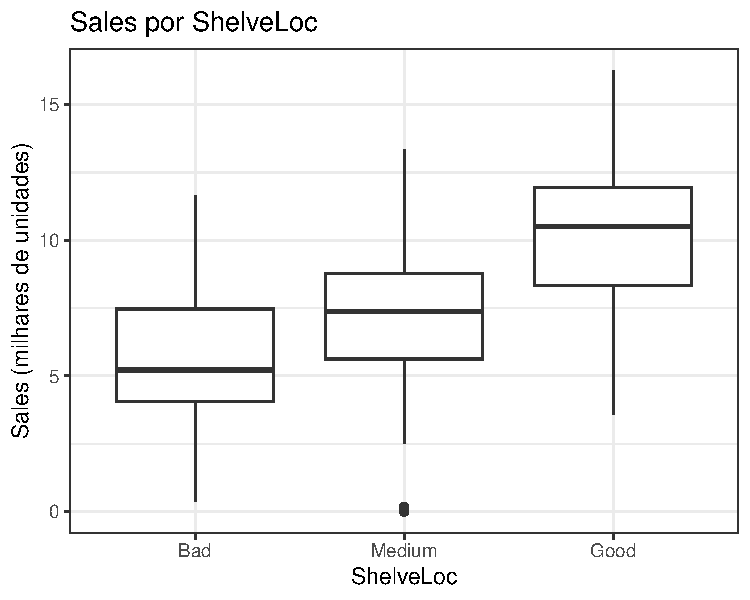
\includegraphics[width=0.7\linewidth]{Relatorio_files/figure-latex/boxplots-1} 

}

\caption{Box-plot das vendas, por qualidade de prateleira.}\label{fig:boxplots}
\end{figure}

Para ShelveLoc Good a mediana das vendas é a maior encontrada, sendo por volta de 12 mil unidades, ou seja,
uma boa qualidade de prateleira tende a possuir maior número de vendas.

Para a ShelveLoc Bad observamos valores médios próximos a 5000, menor mediana encontrada entre os dados. Dessa
forma, percebe-se que uma qualidade ruim resulta em uma quantidade menor de vendas.

Por fim, para a ShelveLoc Medium observamos que ela possui uma mediana que de fato está entre a mediana de
Good e de Bad. Além disso, podemos observar dois outliers, que feita a analise foram identificados sendo os valores 0.16 e 0,
que são valores muito menores que o menor valor próximo a mediana para o grupo Medium.

\subsubsection{Matriz de correlação e dispersão}\label{matriz-de-correlauxe7uxe3o-e-dispersuxe3o}

\begin{figure}[H]

{\centering 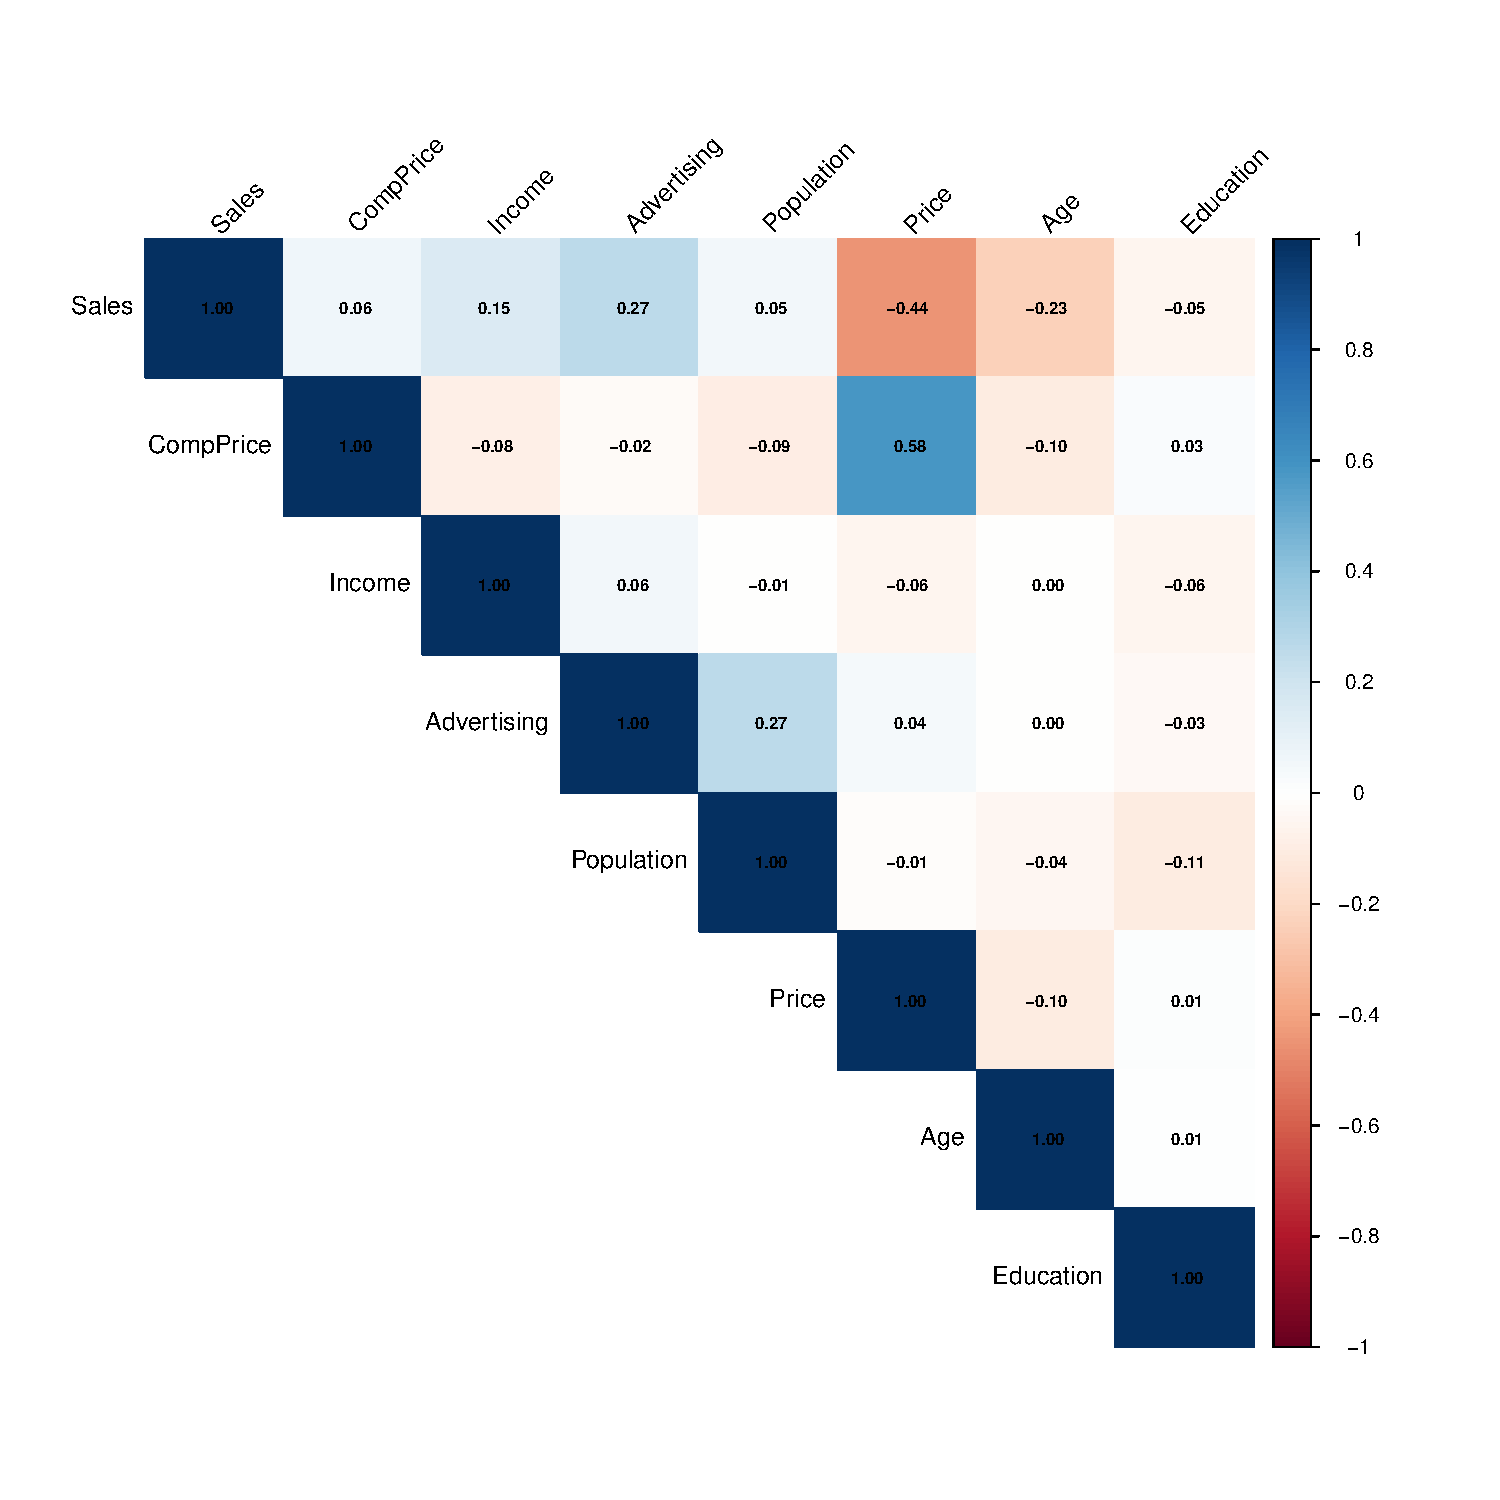
\includegraphics[width=0.72\linewidth]{Relatorio_files/figure-latex/corrplot-1} 

}

\caption{Matriz de correlações entre as variáveis quantitativas.}\label{fig:corrplot}
\end{figure}

\begin{figure}[H]

{\centering 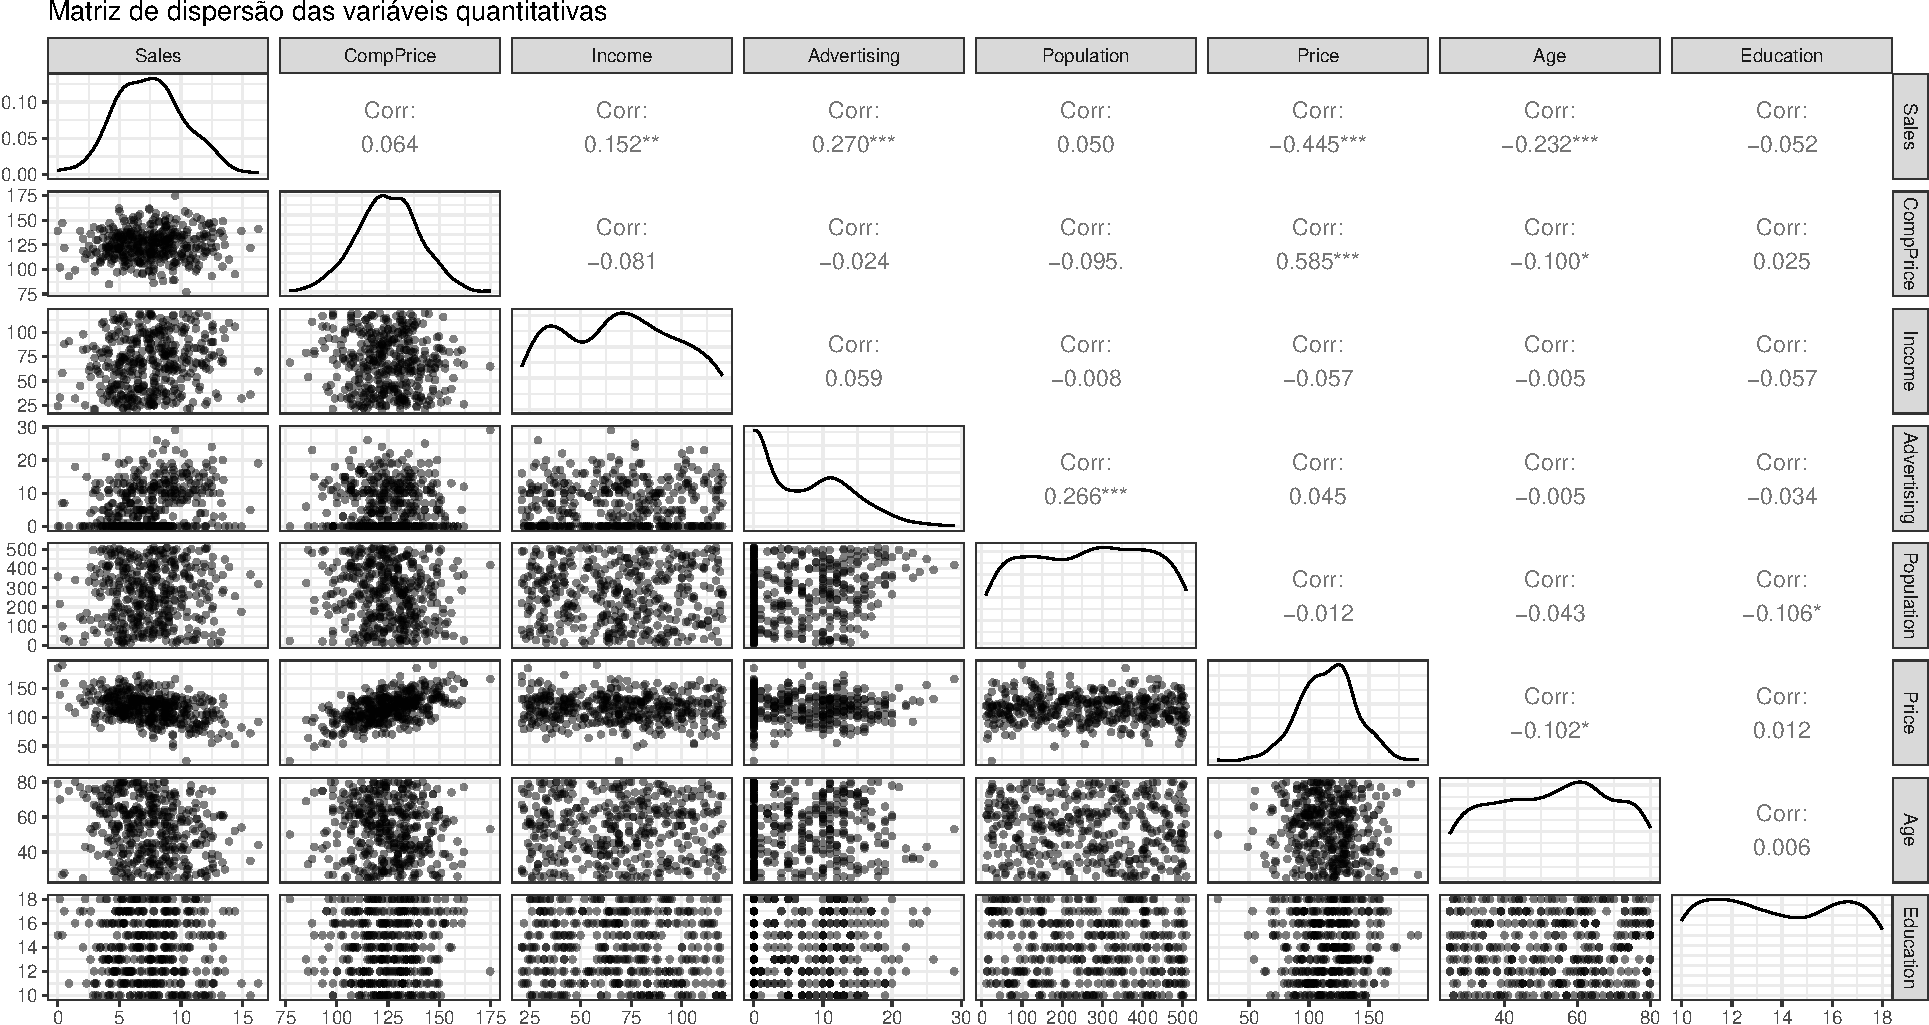
\includegraphics[width=1\linewidth]{Relatorio_files/figure-latex/ggpairs-1} 

}

\caption{Matriz de dispersão par a par.}\label{fig:ggpairs}
\end{figure}

(texto interpretando as correlações --- pode ser escrito em conjunto, pois a leitura costuma ficar mais fácil para quem produziu as estatísticas descritivas)

\subsection{Modelo inicial: todas as variáveis explicativas}\label{modelo-inicial-todas-as-variuxe1veis-explicativas}

\begin{longtable}[]{@{}lrrrr@{}}
\caption{\label{tab:modeloInicial}Tabela de coeficientes do modelo inicial.}\tabularnewline
\toprule\noalign{}
& Estimate & Std. Error & t value & Pr(\textgreater\textbar t\textbar) \\
\midrule\noalign{}
\endfirsthead
\toprule\noalign{}
& Estimate & Std. Error & t value & Pr(\textgreater\textbar t\textbar) \\
\midrule\noalign{}
\endhead
\bottomrule\noalign{}
\endlastfoot
(Intercept) & 5.661 & 0.603 & 9.380 & 0.000 \\
CompPrice & 0.093 & 0.004 & 22.378 & 0.000 \\
Income & 0.016 & 0.002 & 8.565 & 0.000 \\
Advertising & 0.123 & 0.011 & 11.066 & 0.000 \\
Population & 0.000 & 0.000 & 0.561 & 0.575 \\
Price & -0.095 & 0.003 & -35.700 & 0.000 \\
ShelveLocGood & 4.850 & 0.153 & 31.678 & 0.000 \\
ShelveLocMedium & 1.957 & 0.126 & 15.516 & 0.000 \\
Age & -0.046 & 0.003 & -14.472 & 0.000 \\
Education & -0.021 & 0.020 & -1.070 & 0.285 \\
UrbanYes & 0.123 & 0.113 & 1.088 & 0.277 \\
USYes & -0.184 & 0.150 & -1.229 & 0.220 \\
\end{longtable}

\begin{longtable}[]{@{}lr@{}}
\caption{\label{tab:modeloInicial}Métricas de ajuste do modelo inicial.}\tabularnewline
\toprule\noalign{}
Metrica & Valor \\
\midrule\noalign{}
\endfirsthead
\toprule\noalign{}
Metrica & Valor \\
\midrule\noalign{}
\endhead
\bottomrule\noalign{}
\endlastfoot
\(R^2\) & 0.873 \\
\(R^2\) ajustado & 0.870 \\
Erro padrão residual & 1.019 \\
Número de observações & 400.000 \\
\end{longtable}

(texto: R² e significância dos coeficientes)

\subsection{Testes de hipótese e multicolinearidade (VIF)}\label{testes-de-hipuxf3tese-e-multicolinearidade-vif}

(texto: resultado dos testes t individuais, teste F conjunto e discussão sobre o VIF --- há ou não multicolinearidade relevante?)

\subsection{Seleção do modelo final}\label{seleuxe7uxe3o-do-modelo-final}

(texto justificando o modelo final escolhido)

\subsection{Diagnóstico do modelo selecionado}\label{diagnuxf3stico-do-modelo-selecionado}

\subsubsection{Pontos atípicos, de alavanca e influentes}\label{pontos-atuxedpicos-de-alavanca-e-influentes}

\subsubsection{Impacto da remoção dos pontos influentes}\label{impacto-da-remouxe7uxe3o-dos-pontos-influentes}

\subsection{Regressão com variáveis dummy}\label{regressuxe3o-com-variuxe1veis-dummy}

\begin{verbatim}
# Colega 2:
# incluir ShelveLoc, Urban e US no modelo
# discutir a categoria de referência
\end{verbatim}

\subsection{Comparação geral dos modelos}\label{comparauxe7uxe3o-geral-dos-modelos}

\section{Previsões}\label{previsuxf5es}

\subsection{Intervalo de confiança para o valor médio esperado}\label{intervalo-de-confianuxe7a-para-o-valor-muxe9dio-esperado}

(texto de interpretação prática)

\subsection{Intervalo de predição para uma nova observação}\label{intervalo-de-prediuxe7uxe3o-para-uma-nova-observauxe7uxe3o}

(texto de interpretação prática)

\section{Conclusão}\label{conclusuxe3o}

(síntese: principais fatores associados às vendas, qualidade do modelo, limitações e distinção prática entre intervalo de confiança e intervalo de predição)







\bibliographystyle{RS}
\bibliography{modeloUFCG.bib}


\end{document}
